\documentclass[sigconf]{acmart}

% Remove/adjust for your submission venue as needed.
% \settopmatter{printacmref=false} % Removes ACM Reference Format
% \renewcommand\footnotetextcopyrightpermission[1]{} % removes copyright text

\usepackage{lmodern}
\usepackage{tabularx}
\usepackage{booktabs}
\usepackage{url}
\usepackage{tikz}
\usetikzlibrary{arrows.meta,positioning}

%\title{Towards Secure, Multitenant, Vendor-Neutral Enterprise RAG on Shared Infrastructure}
\title{Securing the Agent: Vendor-Neutral, Multitenant Enterprise Retrieval and Tool Use}

\author{Varsha Prasad}
\affiliation{%
  \institution{Red Hat AI}
  \city{Boston}
  \country{USA}
}
\email{vnarsing@redhat.com}

\author{Francisco Javier Arceo}
\affiliation{%
  \institution{Red Hat AI}
  \city{Boston}
  \country{USA}
}
\email{farceo@redhat.com}

\begin{abstract}
Retrieval-Augmented Generation (RAG) and agentic AI systems are increasingly prevalent in enterprise AI deployments. However, real enterprise environments introduce challenges largely absent from academic treatments and consumer-facing APIs: multiple tenants with heterogeneous data, strict access-control requirements, regulatory compliance, and cost pressures that demand shared infrastructure.

A fundamental problem underlies existing RAG architectures in these settings: dense retrieval ranks documents by semantic similarity, not by authorization---so a query from one tenant can surface another tenant's confidential data simply because it is the nearest neighbor. We formalize this gap and analyze additional failure modes---including tool-mediated disclosure, context accumulation across turns, and client-side orchestration bypass---that arise when agentic systems conflate relevance with authorization. To address these challenges, we introduce a layered isolation architecture combining policy-aware ingestion, retrieval-time gating, and shared inference, enforced through server-side agentic orchestration. Unlike client-side agent patterns, this approach centralizes tool execution, state management, and policy enforcement on the server, creating natural enforcement points for multitenant isolation and eliminating per-tenant infrastructure duplication.

Our open-source implementation using Llama Stack---a vendor-neutral framework realizing the Responses API paradigm with server-side multi-turn orchestration---demonstrates that secure multitenancy, cost-efficient resource sharing, and autonomous agent capabilities are simultaneously achievable on shared infrastructure, enabling enterprise deployment of agentic AI with systematic behavioral control.
\end{abstract}

% TODO: update ACM classification.
\begin{CCSXML}
<ccs2012>
 <concept>
  <concept_id>10010147.10010257</concept_id>
  <concept_desc>Computing methodologies~Machine learning</concept_desc>
  <concept_significance>300</concept_significance>
 </concept>
 <concept>
  <concept_id>10002951.10003227.10003351</concept_id>
  <concept_desc>Information systems~Data management systems</concept_desc>
  <concept_significance>100</concept_significance>
 </concept>
</ccs2012>
\end{CCSXML}
\ccsdesc[300]{Computing methodologies~Machine learning}
\ccsdesc[100]{Information systems~Data management systems}

\keywords{Llama Stack, Kubernetes operator, LLM systems, MLOps, LLMOps}

\begin{document}
\maketitle

\section{Introduction}
\subsection{Motivation}
Enterprise adoption of generative AI has evolved beyond simple prompt-response interactions toward agentic systems---AI applications that autonomously reason, use tools, retrieve information, and execute multi-step workflows to accomplish complex tasks~\cite{yao2023react,schick2023toolformer,karpas2022mrkl}.
This evolution reflects a fundamental shift: rather than treating large language models (LLMs) as sophisticated text generators, organizations now deploy them as reasoning engines capable of taking actions in the world.

An API-first paradigm for these systems is to unify multi-turn inference, tool use, and retrieval behind a single endpoint.
OpenAI's Responses API has emerged as a de facto interface pattern for building such systems by providing a unified interface for chat-style inference, tool invocation, retrieval tools, and stateful workflows~\cite{openaiResponsesAPI}.
In parallel, open implementations increasingly expose OpenAI-compatible endpoints to decouple applications from a specific model provider.

However, real-world enterprise deployments differ sharply from the assumptions embedded in consumer-facing APIs and many academic prototypes.
Enterprise environments exhibit characteristics that demand specialized architectural consideration:
\begin{itemize}
  \item \textbf{Multiple tenants:} distinct business units, customers, or partners served from shared infrastructure, with strict isolation requirements.
  \item \textbf{Heterogeneous data:} document collections vary in format, sensitivity classification, and access requirements.
  \item \textbf{Strict access control:} regulatory frameworks require fine-grained governance with auditable access patterns.
  \item \textbf{Operational control:} visibility into agent behavior, tool execution sequences, and data access patterns is required for debugging and compliance, consistent with lessons from production ML engineering~\cite{amershi2019se4ml}.
  \item \textbf{Vendor independence:} lock-in to a single AI provider creates business risk; enterprises require on-prem and hybrid options.
\end{itemize}

Na\"{\i}ve approaches to addressing these requirements replicate the entire agentic stack per tenant: separate vector stores, dedicated inference endpoints, and isolated tool configurations.
This strategy incurs substantial costs --- infrastructure scales linearly with tenants rather than with actual usage --- and creates operational fragmentation that amplifies common ML systems maintenance risks~\cite{sculley2015hiddentechnicaldebt}.

\subsection{Problem statement}
This paper addresses a fundamental tension in enterprise agentic AI deployment:

\begin{quote}
Autonomous agents require flexible tool access and multi-turn reasoning capabilities, yet enterprise environments demand strict tenant isolation and policy enforcement---requirements that existing agentic architectures cannot simultaneously satisfy.
\end{quote}

Standard agentic AI deployments exhibit security assumptions incompatible with enterprise multitenancy:
\begin{enumerate}
  \item \textbf{Client-side orchestration:} the application manages the inference--tool--inference loop, distributing security-critical logic to potentially untrusted clients and increasing operational complexity~\cite{amershi2019se4ml}.
  \item \textbf{Homogeneous data access:} retrieval stacks assume uniform access to a corpus; dense retrieval methods (e.g., DPR) optimize similarity ranking rather than authorization~\cite{karpukhin2020dpr}.
  \item \textbf{Implicit trust boundaries:} tool execution is often treated as a capability extension without systematic verification of who may invoke tools or consume tool outputs, despite the centrality of tool use in modern agent designs~\cite{yao2023react,schick2023toolformer,karpas2022mrkl}.
  \item \textbf{Stateless isolation:} requests are treated independently, ignoring how conversation state and cached tool results can leak across boundaries; such hidden couplings are a classic source of ML systems fragility~\cite{sculley2015hiddentechnicaldebt}.
\end{enumerate}

In multitenant settings, these assumptions create serious vulnerabilities.
A document highly similar to a query may belong to a different tenant.
A tool call may access resources outside the user's authorization scope.
Conversation history may accumulate context that crosses security boundaries.

\subsection{Contributions}
This paper makes the following contributions:
\begin{enumerate}
  \item We formalize the problem of \emph{multitenant enterprise RAG} under shared infrastructure, showing why semantic similarity alone (as used by dense retrievers and ANN indexes) is insufficient to enforce isolation and authorization~\cite{karpukhin2020dpr,johnson2017faiss}.

  \item We analyze failure modes of existing RAG and agentic systems in multitenant settings, including cross-tenant retrieval leakage, unauthorized context construction, and policy violations arising from client-side orchestration.

  \item We propose a layered isolation architecture for enterprise RAG that combines policy-aware ingestion, retrieval-time gating, and shared inference to achieve strict tenant isolation without per-tenant duplication of storage or models.

  \item We introduce server-side orchestration as a unifying enforcement layer that centralizes retrieval, tool execution, and state management, reducing the trusted computing base for secure multitenant RAG and aligning with production ML engineering best practices~\cite{sculley2015hiddentechnicaldebt,amershi2019se4ml}.

  \item We present an open-source, vendor-neutral framework based on Llama Stack~\cite{llamastack} and Kubernetes deployment via an operator~\cite{llamastackk8soperator,burns2016borg} that enables pluggable models, vector stores, and tools, demonstrating the feasibility of secure multitenant RAG on shared infrastructure.
\end{enumerate}

\paragraph{Primary sources.}
Llama Stack~\cite{llamastack}: \url{https://github.com/llamastack/}.\\
Kubernetes operator~\cite{llamastackk8soperator}: \url{https://github.com/llamastack/llama-stack-k8s-operator}.

\section{Background and Related Work}
\subsection{The evolution of LLM application architectures}
LLM application architectures have evolved through distinct phases, each introducing new capabilities and security considerations.
\textbf{Completion APIs} exposed simple prompt\,$\rightarrow$\,text interfaces with perimeter-oriented security.

\textbf{Retrieval-augmented generation (RAG)}~\cite{lewis2020rag} introduced retrieval and new attack surfaces such as retrieval manipulation and context poisoning.
\textbf{Dense retrieval and learned retrievers} (e.g., DPR~\cite{karpukhin2020dpr} and retrieval-augmented pretraining such as REALM~\cite{guu2020realm}) established the core technical basis for modern RAG.
\textbf{Vector search infrastructure} (e.g., FAISS~\cite{johnson2017faiss}) enabled ANN retrieval at scale.
\textbf{Tool-using agents}~\cite{yao2023react,schick2023toolformer,karpas2022mrkl} extended LLMs with tool calls and an inference\,$\rightarrow$\,tool\,$\rightarrow$\,inference loop.
\textbf{Autonomous multi-step agents} execute multi-tool workflows with limited human oversight.
In multitenant deployments, isolation must span retrieval, tool invocation, state accumulation, and orchestration.
Agentic AI systems evolved from prompt-response APIs to autonomous reasoning engines that use tools, retrieve information, and execute multi-step workflows~\cite{yao2023react,schick2023toolformer,karpas2022mrkl,xi2023rise}. The Responses API paradigm~\cite{openaiResponsesAPI,openresponses} unifies these capabilities but assumes single-tenant deployment. Enterprise multitenancy requires policy-aware tool execution, stateful conversation management, and orchestration controls. Production ML systems require systematic lifecycle management~\cite{mlflow} and experience operational fragility when security invariants are distributed across components~\cite{sculley2015hiddentechnicaldebt,amershi2019se4ml}---challenges amplified in agentic deployments where reasoning, retrieval, and tool execution interleave autonomously.

\section{Multitenant Agentic AI: Challenges and Solutions}
\label{sec:challenges-solutions}

We formalize the multitenant agentic AI environment: tenants ($T$) share infrastructure, each with associated data, users, tools, and policies. Agent execution follows the tool-using pattern~\cite{yao2023react,karpas2022mrkl}: $E = [(i_1, \phi_1, r_1), (i_2, \phi_2, r_2), \dots, (i_n, \emptyset, r_n)]$.

Key threats include cross-tenant data leakage via retrieval, tool-mediated disclosure, context accumulation attacks, and client-side orchestration bypass. Standard agentic deployments exhibit fundamental incompatibilities with enterprise multitenancy.

\subsection{Core failure modes}

\textbf{Similarity-authorization gap:} RAG frameworks retrieve by semantic similarity~\cite{karpukhin2020dpr,johnson2017faiss}, not authorization. For tenants $T_A$ and $T_B$ sharing corpus $D = D_A \cup D_B$, similarity-based retrieval cannot enforce tenant isolation without an authorization predicate: $\mathcal{R}(q,u) = \{ d \in D : \mathrm{sim}(q,d) > \theta \wedge P(u,d) = \mathrm{permit} \}$.

\textbf{Tool-mediated disclosure:} Agents invoke tools with agent credentials rather than end-user authorization, potentially accessing unauthorized data across tenant boundaries.

\textbf{Context accumulation:} Multi-turn conversations persist context without per-turn policy re-validation, enabling cross-tenant data leakage.

\textbf{Client-side bypass:} When orchestration runs client-side, malicious clients can skip authorization checks, manipulate tool invocation, or extract unauthorized data.

These failures stem from distributing security-critical logic outside the trust boundary~\cite{sculley2015hiddentechnicaldebt,amershi2019se4ml}.

\subsection{Layered isolation solution}
We propose a three-layer architecture with server-side orchestration:

\textbf{Layer 1: Policy-aware ingestion.} Tenant metadata attached at ingestion: $\mathcal{I}(d, t) \rightarrow D_t$ tags document $d$ with tenant $t$'s attributes.

\textbf{Layer 2: Retrieval gating.} Two-tier enforcement: resource-level authorization before search and chunk-level filtering after retrieval, composing similarity search with authorization predicates.

\textbf{Layer 3: Shared inference.} LLM layer shared across tenants with isolation enforced at input construction, reducing cost from $O(N \cdot M)$ to $O(M)$.

\subsection{Server-side orchestration as enforcement layer}
Server-side orchestration centralizes retrieval, tool execution, and state management within the trust boundary, eliminating client-side bypass risks. This design aligns with tool-using agent formulations~\cite{yao2023react,karpas2022mrkl} while enabling centralized policy enforcement, audit logging, and state isolation.

We propose a three-layer architecture that directly addresses the failure modes identified in Section~\ref{sec:common-limitations}: policy-aware ingestion, retrieval-time gating, and shared inference.

\subsection{Policy-aware ingestion (Layer 1)}
Tenant metadata must be attached at document ingestion time, not retrofitted.
This reduces the risk of accidental cross-tenant coupling and missing invariants during system evolution~\cite{sculley2015hiddentechnicaldebt}.
Define an ingestion function $\mathcal{I}(d, t) \rightarrow D_t$ that tags document $d$ with tenant $t$'s attributes so that every chunk inherits ownership metadata.
In Llama Stack, when files are attached to vector stores, the \texttt{attributes} parameter carries tenant ownership, classification, and access policy; these are stored as chunk metadata.

\subsection{Retrieval gating (Layer 2)}
Retrieval is gated in two tiers.
\textbf{(1) Resource-level ABAC:} before any search, the system checks that the user is authorized to read the vector store; if not, no search is performed.
\textbf{(2) Chunk-level metadata filtering:} after retrieval, structured filters are applied on chunk metadata so that only documents satisfying the policy are admitted.
This composes similarity search (dense retrieval~\cite{karpukhin2020dpr} over ANN indexes~\cite{johnson2017faiss}) with a mandatory authorization predicate:
\[
\mathcal{R}(q,u) = \{ d \in D : \mathrm{sim}(q,d) > \theta \wedge P(u,d) = \mathrm{permit} \}.
\]
Backends such as Elasticsearch and SQL-backed vector stores can support predicate pushdown for efficiency on large corpora; otherwise, post-retrieval gating still enforces the semantic/authorization separation.

\subsection{Shared inference (Layer 3)}
The LLM inference layer is shared across tenants; the model itself does not require per-tenant isolation, only the context fed to it.
Because layers 1 and 2 ensure that only authorized documents and tool results enter the prompt, the inference layer can be safely shared.
At the serving layer, modern systems show that batching, scheduling, and memory management dominate throughput and latency for generative transformers~\cite{yu2022orca,kwon2023vllm}.
With $N$ tenants and $M$ model endpoints, cost scales as $O(M)$ rather than $O(N \cdot M)$.

\section{Server-Side Orchestration as Enforcement Layer}
\label{sec:server-side}

Server-side orchestration is essential for multitenant security: it centralizes retrieval, tool execution, and state management, reducing the trusted computing base and addressing failure modes in Section~\ref{sec:common-limitations}.
This design also aligns with the execution structure implied by tool-using agent formulations~\cite{yao2023react,karpas2022mrkl}.

\subsection{The case against client-side orchestration}
In client-side patterns, the client controls the inference--tool--inference loop.
A compromised or buggy client can skip retrieval filters, invoke unauthorized tools, or accumulate cross-tenant context.
Formally, client-side orchestration expands the TCB to include untrusted client code, so server-side security invariants cannot be enforced from the server alone.
This is consistent with broader findings that ML systems become fragile when critical invariants are distributed across components without clear ownership or enforcement points~\cite{sculley2015hiddentechnicaldebt,amershi2019se4ml}.

\subsection{Server-side orchestration in Llama Stack}
Llama Stack implements the Responses API with the full loop executed on the server~\cite{llamastack,openaiResponsesAPI}.
Tool execution (\texttt{file\_search}, \texttt{web\_search}, MCP, and function tools) runs inside the server trust boundary, and state is managed server-side with tenant-scoped access control.
Streaming events expose tool calls and text deltas, improving observability in line with production ML monitoring and governance needs~\cite{amershi2019se4ml}.

\begin{figure}[t]
    \centering
    \resizebox{\columnwidth}{!}{%
    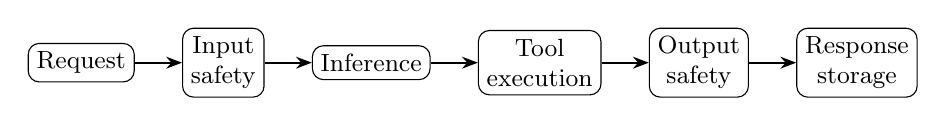
\begin{tikzpicture}[
      box/.style={draw, rounded corners, align=center, inner sep=3pt, font=\small},
      arrow/.style={-{Stealth[length=2.0mm]}, thick}
    ]
      \node[box] (req) {Request};
      \node[box, right=6mm of req] (in) {Input\\safety};
      \node[box, right=6mm of in] (inf) {Inference};
      \node[box, right=6mm of inf] (tool) {Tool\\execution};
      \node[box, right=6mm of tool] (out) {Output\\safety};
      \node[box, right=6mm of out] (store) {Response\\storage};
      \draw[arrow] (req) -- (in);
      \draw[arrow] (in) -- (inf);
      \draw[arrow] (inf) -- (tool);
      \draw[arrow] (tool) -- (out);
      \draw[arrow] (out) -- (store);
    \end{tikzpicture}%
    }
    \caption{Server-side orchestration flow: every step runs inside the server trust boundary.}
    \label{fig:orchestration-flow}
  \end{figure}

\subsection{Enforcement points}
Table~\ref{tab:enforcement} maps each failure mode from Section~\ref{sec:common-limitations} to the enforcement point that mitigates it.
\textbf{Server-side orchestration:} Centralizes retrieval, tool execution, and state management within the trust boundary, eliminating client-side bypass risks while enabling policy enforcement and audit logging~\cite{yao2023react,karpas2022mrkl}.

\begin{table}[t]
  \centering
  \small
  \setlength{\tabcolsep}{3pt}
  \renewcommand{\arraystretch}{1.1}
  \begin{tabularx}{\columnwidth}{@{}l|X@{}}
  \toprule
  Failure mode & Enforcement point \\
  \midrule
  Cross-tenant retrieval leakage & Layer 2 retrieval gating (ABAC + metadata filters) \\
  \midrule
  Context accumulation & Tenant-scoped state storage and per-turn authorization \\
  \midrule
  Tool-mediated disclosure & Server-side tool execution with authorization propagation \\
  \midrule
  Client-side bypass & Server-side orchestration (reduced TCB) \\
  \midrule
  Audit failure & Server-side telemetry and tracing \\
  \bottomrule
  \end{tabularx}
  \caption{Mapping from failure modes to architectural enforcement points.}
  \label{tab:enforcement}
\end{table}

\section{Llama Stack Implementation}
\label{sec:implementation}

Llama Stack~\cite{llamastack} provides an open-source implementation of the proposed architecture. Unlike client-side orchestration libraries, it executes the complete agentic control loop server-side, creating natural enforcement points for multitenancy~\cite{openaiResponsesAPI}.

The framework implements provider abstraction enabling pluggable inference (vLLM~\cite{kwon2023vllm}, Ollama, OpenAI), vector stores (Chroma, pgvector, Elasticsearch), and tools (file\_search, web\_search, Model Context Protocol~\cite{mcp}). This design enables integration with emerging agent communication standards~\cite{a2a} and systematic tool orchestration patterns. Together, Llama Stack, vLLM, and open models like gpt-oss~\cite{openai2025gptoss120bgptoss20bmodel} provide a complete open-source alternative to proprietary agentic AI platforms, enabling enterprise deployment with full control over the inference stack and creating opportunities for systematic agent evaluation~\cite{jimenez2024swebench,liu2024agentbench}.

The Kubernetes Operator~\cite{llamastackk8soperator} supports deployment topologies from shared instances with logical isolation to per-tenant deployments with namespace isolation. Authorization is enforced at API routes, routing resolution, and tool execution, with tenant-scoped state storage preventing cross-tenant leakage.

Authorization is enforced at API routes, routing resolution, and tool execution, with tenant-scoped state storage and per-turn policy checks preventing cross-tenant leakage.

Second, the framework adopts a pluggable provider model. Each API is implemented by interchangeable providers that share a common interface, enabling vendor independence and hybrid deployments across on-premise and cloud environments.

Third, Llama Stack implements server-side agentic orchestration. The full agentic execution loop—including inference, tool invocation, and subsequent inference—executes within the server trust boundary. This design contrasts with client-side orchestration approaches and enables centralized enforcement of access control, safety policies, and execution constraints.

Finally, the framework introduces a distribution model. Pre-configured combinations of APIs and providers are packaged as distributions, enabling turnkey deployment while preserving flexibility for customization and provider substitution.

\subsection{Layered Architecture}
Llama Stack follows a layered architecture that separates concerns across distinct tiers, as illustrated in Figure~\ref{fig:architecture}. At the top, an HTTP/REST layer handles request routing, authentication, quota enforcement, and streaming. Beneath this layer, a set of domain-specific APIs expose functionality for inference, agentic execution, vector I/O, safety, and tool integration.

A routing layer mediates between API calls and concrete provider implementations, resolving logical resource identifiers (e.g., model identifiers or vector store identifiers) to physical provider instances. Below this, a provider layer encapsulates both inline providers executing in-process and remote providers that adapt external services. Persistent state is maintained in a storage layer comprising key–value stores, relational stores, and vector databases.

This separation enables independent evolution of APIs, providers, and storage backends while preserving a unified control plane for policy enforcement.

\subsection{Core APIs and Agentic Execution}
Llama Stack defines a comprehensive set of APIs covering the full lifecycle of agentic applications, including inference, agents, vector I/O, safety, tools, file management, and evaluation. Each API is designed with multitenancy as a first-class concern, enabling tenant-scoped resource management and access control.

The Agents API, which implements the OpenAI Responses API paradigm, is particularly significant for multitenant agentic systems. Unlike traditional chat completion APIs that terminate after a single inference call, the Responses API orchestrates complete agentic workflows. A single request may trigger multiple inference calls, tool executions, safety checks, and state transitions before producing a final response.

All such operations are executed within the server boundary. Conversation state is retrieved and persisted server-side, tools are invoked under centralized authorization, and safety guardrails are applied at each step. This design ensures that intermediate context, tool outputs, and execution state remain subject to uniform access control policies.

\subsection{Provider Architecture}
Extensibility in Llama Stack is achieved through its provider architecture. Each API may be backed by multiple providers, which are categorized as inline or remote. Inline providers execute within the Llama Stack process and are suitable for sensitive operations requiring in-process execution. Remote providers adapt external inference engines, vector databases, or services through standardized interfaces.

This separation enables hybrid deployments in which sensitive data paths remain local while computationally intensive operations are delegated to scalable external services. Crucially, provider substitution is transparent to clients, as all interactions occur through the unified API layer.

\subsection{Routing Layer}
The routing layer dispatches API requests to provider instances based on logical resource identifiers. For example, inference requests are routed according to model identifiers, while vector queries are routed based on vector store identifiers. This indirection enables fine-grained control over resource access and placement.

From a multitenancy perspective, the routing layer serves as a critical enforcement point. Routing decisions can incorporate authorization checks, tenant identity, and policy constraints before delegating requests to providers. Different tenants may thus be routed to distinct provider instances or storage backends while sharing the same API surface.

\subsection{Distribution Model}
A distribution packages a specific set of APIs, provider configurations, and registered resources into a deployable unit. Distributions support turnkey deployment for common scenarios, environment-specific configuration (e.g., development versus production), and seamless provider substitution without application changes.

By decoupling application logic from provider selection, the distribution model enables organizations to evolve their infrastructure and vendor choices while preserving stable interfaces for agentic applications.

\subsection{Access Control Framework}
Llama Stack includes a declarative, policy-based access control framework that evaluates authorization decisions at runtime. Policies specify permitted and forbidden actions over resource scopes, with conditions based on user identity, resource attributes, and ownership relationships.

Authorization checks are enforced at multiple layers, including API routes, routing table resolution, and tool execution. A default-deny model ensures that access is only granted when explicitly permitted by policy. This design enables consistent enforcement across inference, retrieval, and agentic execution.

\subsection{Server Architecture}
The Llama Stack server is implemented atop a modern asynchronous web framework and provides OpenAI-compatible endpoints for inference and agentic execution. Authentication middleware supports pluggable identity providers, while quota management enables per-principal rate limiting and usage tracking. Streaming execution is supported for long-running agentic workflows, and telemetry integration enables end-to-end observability.

Importantly, all agentic orchestration occurs within the server process, enabling comprehensive audit logging of inference calls, tool executions, and data access events.

\subsection{Implications for Multitenant Agentic AI}
Taken together, these architectural choices yield several properties essential for multitenant enterprise deployments. First, centralized orchestration creates uniform enforcement points for access control and policy compliance. Second, provider-level isolation enables tenant-specific routing while preserving shared infrastructure. Third, server-managed state prevents cross-tenant context leakage across multi-turn interactions. Finally, centralized execution enables comprehensive auditing and compliance monitoring.

These properties form the foundation for the layered isolation architecture described in the following section, where we show how policy-aware ingestion, retrieval gating, and server-side orchestration can be composed to achieve secure, cost-efficient multitenant agentic AI.


\subsection{High-level architecture}
We propose a layered architecture for secure multitenant agentic AI with an authentication layer, a server-side agentic orchestrator, policy evaluation, and a shared-but-logically-isolated vector store.

\begin{figure}[t]
  \centering
  \resizebox{\columnwidth}{!}{%
  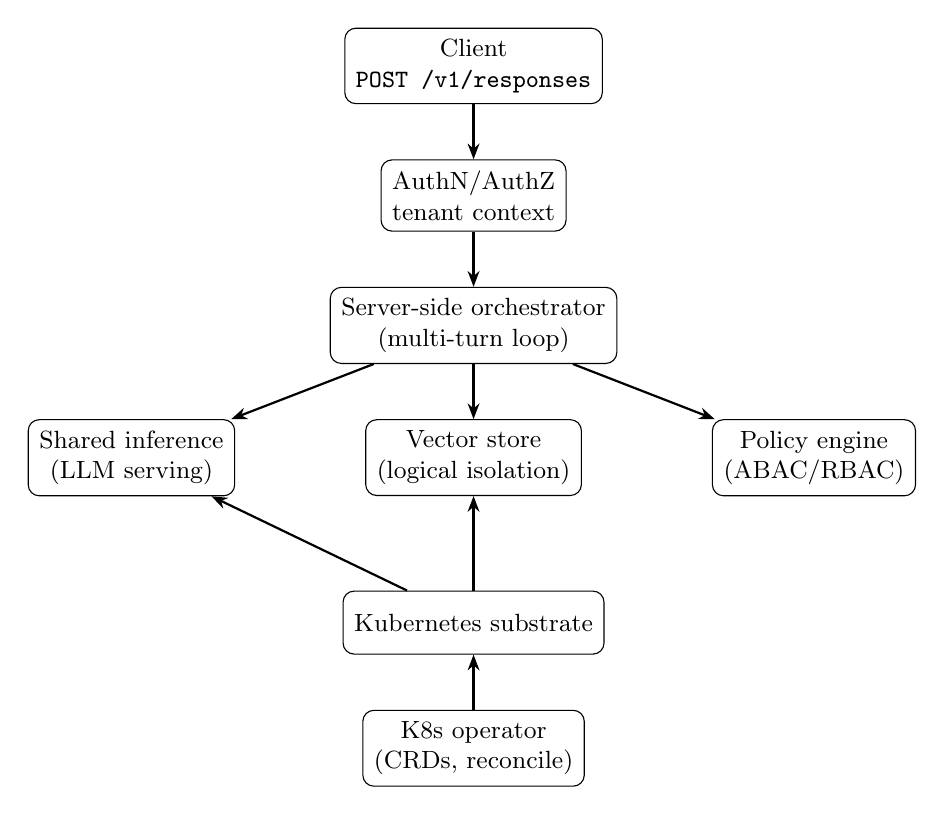
\begin{tikzpicture}[
    box/.style={draw, rounded corners, align=center, inner sep=4pt, minimum height=8mm, font=\small},
    arrow/.style={-{Stealth[length=2.0mm]}, thick}
  ]
    \node[box] (client) {Client\\\texttt{POST /v1/responses}};
    \node[box, below=7mm of client] (auth) {AuthN/AuthZ\\tenant context};
    \node[box, below=7mm of auth] (orch) {Server-side orchestrator\\(multi-turn loop)};

    \node[box, below left=7mm and 12mm of orch] (infer) {Shared inference\\(LLM serving)};
    \node[box, below=7mm of orch] (vec) {Vector store\\(logical isolation)};
    \node[box, below right=7mm and 12mm of orch] (policy) {Policy engine\\(ABAC/RBAC)};

    \node[box, below=12mm of vec] (k8s) {Kubernetes substrate};
    \node[box, below=7mm of k8s] (op) {K8s operator\\(CRDs, reconcile)};

    \draw[arrow] (client) -- (auth);
    \draw[arrow] (auth) -- (orch);

    \draw[arrow] (orch) -- (infer);
    \draw[arrow] (orch) -- (vec);
    \draw[arrow] (orch) -- (policy);

    \draw[arrow] (op) -- (k8s);
    \draw[arrow] (k8s) -- (infer);
    \draw[arrow] (k8s) -- (vec);
  \end{tikzpicture}%
  }
  \caption{Reference architecture for multitenant enterprise agentic AI on shared Kubernetes infrastructure.}
  \label{fig:architecture}
\end{figure}


\subsection{Authentication and tenant context}
Requests begin with authentication establishing a user and tenant context.
Claims (tenant/namespace, roles/groups, projects) are mapped to authorization attributes and propagated through the request lifecycle.

\subsection{Server-side agentic orchestration}
The orchestrator executes the multi-turn loop server-side: inference, tool-call detection, tool classification, policy evaluation, tool execution, and context construction.
Server-side tools (e.g., \texttt{file\_search}, \texttt{web\_search}, MCP tools) are executed within the trust boundary; client-side function tools are explicitly delegated.

\subsection{Policy-aware ingestion}
Ingestion attaches mandatory metadata (tenant attribution, classification) and records lineage for audit.
Documents without required metadata are rejected.

\subsection{Shared vector store with logical isolation}
A single physical vector index is shared, but each chunk carries tenant and policy metadata.
Retrieval uses query-time predicates (tenant predicates and classification filters) to prevent cross-tenant candidate leakage, separating similarity ranking from authorization checks~\cite{karpukhin2020dpr,johnson2017faiss}.

\subsection{Two-phase retrieval: search and admission}
Phase~1 performs filtered similarity search, grounded in dense retrieval and ANN indexing methods~\cite{karpukhin2020dpr,johnson2017faiss}.
Phase~2 applies policy-based admission; only admitted documents enter the generation context, and denials are logged.

\subsection{Tool execution with policy gating}
Every tool invocation is preceded by policy evaluation over user attributes, tool identity, and parameters.
This is particularly important for agent loops where the model chooses actions and tools iteratively~\cite{yao2023react,schick2023toolformer,karpas2022mrkl}.

\subsection{Shared inference with isolated contexts}
LLM instances are shared across tenants, but each request constructs an isolated context containing only authorized inputs.
Serving efficiency and scheduling are handled by the inference backend; modern LLM serving systems show that batching and memory management dominate throughput~\cite{yu2022orca,kwon2023vllm}.
Because isolation is enforced at ingestion and retrieval, the inference layer itself does not need per-tenant replicas—reducing cost to $O(M)$ model endpoints for $N$ tenants while preserving strict logical isolation.

\subsection{Overview and implementation}
Llama Stack is an open-source framework implementing the Responses API paradigm with server-side orchestration~\cite{llamastack,openaiResponsesAPI}.
It is vendor-neutral via a provider abstraction, and is designed for Kubernetes-native deployment and operator-based lifecycle management~\cite{llamastackk8soperator,burns2016borg}.

\subsection{Responses API implementation}
The Responses API exposes operations to create responses (execute an agent), retrieve responses, list responses, inspect input items, and delete responses; creation supports both streaming and non-streaming modes.
Internally, the implementation converts request input to chat messages and runs the inference--tool loop via a streaming orchestrator or a synchronous path.
Results are persisted through a responses store backed by an authorized SQL layer so that rows are tagged with owner and access attributes and filtered on read by the default ABAC policy.
Streaming events expose reasoning, tool calls, and text deltas, giving operators and auditors fine-grained visibility into agent behavior without requiring client-side instrumentation.

\subsection{Vector store abstraction and filters}
Llama Stack defines a vector store protocol (vector I/O API) implemented by multiple providers (e.g., Chroma, pgvector, Elasticsearch, in-process SQLite).
Each vector store is a logical resource registered in a routing table and subject to the same access control as other resources; creation assigns an owner from the authenticated user.
The protocol supports a structured filter language for query-time metadata constraints: comparison operators (\texttt{eq}, \texttt{ne}, \texttt{gt}, \texttt{gte}, \texttt{lt}, \texttt{lte}) and compound \texttt{and}/\texttt{or} filters.
When the agent uses \texttt{file\_search}, the server applies the user's tenant and policy attributes so that retrieval is gated by both resource-level and chunk-level checks, enabling metadata-driven isolation without requiring a separate physical index per tenant.

\subsection{Attribute-based access control}
Llama Stack supports ABAC-style policies for tenant isolation, role-based capabilities, and classification enforcement.
The access control engine evaluates \texttt{Access\-Rule}s with permit/forbid scopes and optional conditions (e.g., ``user in owners roles'', ``user is owner'', ``resource is unowned''); the default policy permits access when the user is the resource owner or when the user's attributes (roles, teams, projects, namespaces) match the resource's access attributes.
Authorization is enforced at API routes (e.g., \texttt{Route\-Authorization\-Middleware}), at routing table resolution (e.g., before resolving a vector store or model), and at storage read time via \texttt{Authorized\-Sql\-Store}, which builds SQL \texttt{WHERE} clauses from the current user so that tenants only see their own or attribute-matched rows.
JWT or Kubernetes auth providers map external claims (e.g., \texttt{tenant}, \texttt{groups}) into these attributes, so enterprise identity systems can drive isolation without embedding tenant IDs in application logic.

\subsection{Cloud-Native Deployment}
The architectural guarantees described above must be realized on shared infrastructure. Kubernetes has become the de facto substrate for enterprise deployments~\cite{burns2016borg}.

The Llama Stack Kubernetes Operator~\cite{llamastackk8soperator} automates deployment and lifecycle management through custom resources that declaratively specify server configurations, backend connections, and isolation policies. The operator supports multiple deployment topologies:

\begin{itemize}
  \item \textbf{Shared instances}: Single deployment serving multiple tenants with application-level ABAC isolation
  \item \textbf{Per-tenant instances}: Separate deployments in tenant-specific namespaces combining Kubernetes RBAC with application-level policies
  \item \textbf{Hybrid approaches}: High-security tenants receive dedicated instances while lower-sensitivity tenants share infrastructure
\end{itemize}

The operator's provider abstraction enables deployment of heterogeneous inference backends (vLLM~\cite{kwon2023vllm}, Ollama, proprietary endpoints) and vector stores (FAISS~\cite{johnson2017faiss}, ChromaDB, Qdrant) as shared Kubernetes services. Multiple Llama Stack instances reference the same backends, achieving cost savings through infrastructure sharing while maintaining logical isolation through the authorization layer.

This design scales economically: adding tenants requires only logical configuration (authorization policies, database schemas) rather than full infrastructure duplication, crucial for cost-constrained enterprise deployments.

\section{Analysis and Discussion}

The layered isolation architecture addresses core failure modes: similarity retrieval with policy predicates prevents cross-tenant leakage~\cite{karpukhin2020dpr,johnson2017faiss}, centralized tool execution reduces unauthorized access~\cite{yao2023react,schick2023toolformer}, and tenant-scoped storage prevents context accumulation~\cite{sculley2015hiddentechnicaldebt,amershi2019se4ml}.

Performance depends on inference backend efficiency~\cite{kwon2023vllm}. Limitations include ABAC policy complexity at scale, variable metadata filtering performance across backends, and model prior knowledge being orthogonal to RAG isolation.

\section{Conclusion}
Agentic AI systems with autonomous tool use and multi-step reasoning introduce security and compliance challenges that exceed the assumptions in standard client-orchestrated patterns.
We formalized the similarity-authorization gap in agentic retrieval~\cite{karpukhin2020dpr,johnson2017faiss} and analyzed failure modes unique to autonomous agent architectures, including tool-mediated disclosure and client-side orchestration bypass.

Our layered isolation architecture demonstrates that server-side orchestration can serve as a unifying enforcement layer for secure agent behavior, centralizing retrieval, tool execution, and state management to maintain enterprise control over autonomous actions~\cite{sculley2015hiddentechnicaldebt,amershi2019se4ml}.

Llama Stack~\cite{llamastack} demonstrates that vendor-neutral, open-source tooling can enable enterprise-grade agentic multitenancy through provider abstraction and server-side Responses API implementation~\cite{openaiResponsesAPI,openresponses}. Combined with efficient serving infrastructure~\cite{kwon2023vllm} and open models~\cite{openai2025gptoss120bgptoss20bmodel}, this provides a complete alternative to proprietary agentic platforms.

The patterns presented establish a foundation for secure, scalable autonomous agent deployments with systematic behavioral control.

\bibliographystyle{ACM-Reference-Format}
\bibliography{references}

\end{document}
